% Gets the style guide to apply to the document such as font sizes for various wrappers, spacing before and after sections, etc.
% \documentclass[letterpaper,twoside,openright]{document-formatting} %this is for double sided alternating the extra margin on left and right pages
\documentclass[letterpaper,onesided,openright]{document-formatting}
% NOTE THAT THE SECOND LAST LINE OF DOCUMENT-FORMATTING.CLS LETS YOU CHANGE THE CITATION STYLE

% Hides addition of external plugins
% This package is for charsets (default)
\usepackage[utf8]{inputenc}

% The principal package in the AMS-LATEX distribution. It adapts for use in LATEX most of the mathematical features found in AMS-TEX; it is highly recommended as an adjunct to serious mathematical typesetting in LATEX. (https://ctan.org/pkg/amsmath?lang=en)
\usepackage{amsmath}
\usepackage{mathdots}

% better absolute brackets
\usepackage{mathtools}
\DeclarePairedDelimiter\abs{\lvert}{\rvert}%
\DeclarePairedDelimiter\norm{\lVert}{\rVert}%

% Swap the definition of \abs* and \norm*, so that \abs
% and \norm resizes the size of the brackets, and the 
% starred version does not.
\makeatletter
\let\oldabs\abs
\def\abs{\@ifstar{\oldabs}{\oldabs*}}
%
\let\oldnorm\norm
\def\norm{\@ifstar{\oldnorm}{\oldnorm*}}
\makeatother

% Algorithm2e is an environment for writing algorithms. (https://ctan.org/pkg/algorithm2e?lang=en)
\usepackage{algorithm2e}

 % The package builds upon the graphics package, providing a key-value interface for optional arguments to the \includegraphics command. This interface provides facilities that go far beyond what the graphics package offers on its own. (https://ctan.org/pkg/graphicx?lang=en)
\usepackage{graphicx}

% This package is for font and sizing the captions on figures and tables.
\usepackage[labelfont=bf,font={footnotesize,singlespacing}]{caption}

% A LATEX2ε package to help change the style of any or all of LATEX's sectional headers in the article, book, or report classes. Examples include the addition of rules above or below a section title. (https://ctan.org/pkg/sectsty?lang=en)
\usepackage{sectsty}
\sectionfont{\vspace{-0.0em}\large\bfseries\addvspace{-1.5em}}
\subsectionfont{\vspace{-2.0em}\normalsize\bfseries\addvspace{-0.0em}}
\subsubsectionfont{\vspace{-2.0em}\normalsize\bfseries\addvspace{-0.5em}}

% The xr package is used for cross-referencing across multiple independent documents. For example, you would use the xr package if you had two separate files in a project, File1.tex and File2.tex, and you would like to have a reference in File1.tex to something labelled in File2.tex, without including File2.tex in File1.tex. (https://www.overleaf.com/learn/how-to/Cross_referencing_with_the_xr_package_in_Overleaf)
\usepackage{xr}

% The hyperref package is used to handle cross-referencing commands in LATEX to produce hypertext links in the document. (https://ctan.org/pkg/hyperref?lang=en)
\usepackage{hyperref}

% The package enhances LATEX’s cross-referencing features, allowing the format of references to be determined automatically according to the type of reference. (https://ctan.org/pkg/cleveref?lang=en)
\usepackage{cleveref}

% Package to show and highlight code
\usepackage{listings}

% Allow Multicolumn sections
\usepackage{blindtext} % for adding some random text data in sections
\usepackage{multicol} % for making multi column layouts

% To make sure that Latex doesn't reposition tables
\usepackage{float}
\floatstyle{plaintop}
\restylefloat{table}
% \restylefloat{figure}

\usepackage{afterpage}
\usepackage[section]{placeins}

% all figure file names relative to this path
%\graphicspath{ {../Figures/} } %NOT REALLY NEEDED IF YOU JUST DIRECT LINK INSTEAD OF RELATIONAL LINK

%allow right aligned columns
\usepackage{array,booktabs,ragged2e}
\newcolumntype{R}[1]{>{\RaggedLeft\arraybackslash}p{#1}}

%colour table rows
\usepackage{color, colortbl}
\definecolor{Gray}{gray}{0.9}

%%% HELPER CODE FOR DEALING WITH EXTERNAL REFERENCES
\makeatletter
\newcommand*{\addFileDependency}[1]{
  \typeout{(#1)}
  \@addtofilelist{#1}
  \IfFileExists{#1}{}{\typeout{No file #1.}}
}
\makeatother

\newcommand*{\myexternaldocument}[1]{
    \externaldocument{#1}
    \addFileDependency{#1.tex}
    \addFileDependency{#1.aux}
}

%%% END HELPER CODE

% Page numbering
\usepackage{fancyhdr} % to change header and footers

% Redefine plain style, which is used for titlepage and chapter beginnings
% From https://tex.stackexchange.com/a/30230/828
\fancypagestyle{plain}{%
    \renewcommand{\headrulewidth}{0pt}%
    \fancyhf{}%
    % \fancyfoot[R]{\thepage}%
}

\fancypagestyle{noNumber}{%
    \renewcommand{\headrulewidth}{0pt}%
    \fancyhf{}%
    \pagenumbering{alph}
    % \fancyfoot[R]{\thepage}%
}

\fancypagestyle{fancyRoman}{%
    \renewcommand{\headrulewidth}{0pt}%
    \renewcommand{\footrulewidth}{1pt}%
    \fancyhf{}%
    \fancyfoot[R]{\thepage}%
    \pagenumbering{roman}
}

\fancypagestyle{fancyArabic}{%
    \renewcommand{\headrulewidth}{0pt}%
    \renewcommand{\footrulewidth}{1pt}%
    \fancyhf{}%
    \fancyfoot[R]{\thepage}%
    \fancyhead[R]{\raisebox{1.0cm}[0pt][0pt]{\hspace{1.5cm}Jordan D. Lanct\^{o}t}}%
    \pagenumbering{arabic}
}

% Alternating margins support
\usepackage[letterpaper,inner=1.87cm,outer=1.87cm,top=1.87cm,bottom=1.87cm]{geometry}

%% MY COMMANDS
\newcommand{\high}[1]{\text{\raisebox{0.6ex}{$#1$}}}
\newcommand{\higher}[1]{\text{\raisebox{1.5ex}{$#1$}}}
\newcommand{\overbar}[1]{\mkern 1.5mu\overline{\mkern-1.5mu#1\mkern-1.5mu}\mkern 1.5mu}\unskip

\begin{document}

% Title Page
\title{AI-Driven Approaches for Network Resilience: From Attack-Defence Strategies to Cascading Failure Mitigation}
\author{Jordan~D.~~Lanct\^{o}t$^{1}$, Sean~P.~~Cornelius$^{1,2, \dagger}$}
\date{September 2024}

\maketitle
\thispagestyle{noNumber}

{\small
\begin{affiliations}
 \item \, Department of Physics, Toronto Metropolitan University, Toronto, ON M5B 2K3, Canada
 \item[$\dagger$] \, To whom correspondence should be addressed
\end{affiliations}
}

\vspace{3em}
\begin{abstract}
Networked systems, ubiquitous in modern infrastructure, are susceptible to cascading failures and targeted attacks. This research investigates network robustness through three interconnected studies. First, we explore the application of deep reinforcement learning (DRL) in network attack and defense scenarios. Neural network embedding frameworks are employed to discover vulnerable nodes, while DRL agents are developed to either dismantle networks efficiently or defend against such attacks through partial network concealment. Our early findings reveal a surprising disadvantage for defensive strategies across various network configurations.\\

Building on these insights, we will examine cascading failures using the Abelian sandpile model as a framework. We will simulate and analyze the efficacy of targeted interventions, including strategic sand dropping and link rewiring, to mitigate avalanche effects in networks. This approach will provide a deeper understanding of failure propagation dynamics and potential preventive measures.\\

Finally, we will extend our investigation of the Abelian sandpile model by applying DRL techniques to refine and optimize the aforementioned failure mitigation strategies. This advanced approach will aim to develop more sophisticated, adaptive methods for maintaining network integrity under diverse stress conditions. Through this comprehensive analysis of network vulnerabilities, failure mechanisms, and mitigation strategies, we will contribute fundamental insights into enhancing the robustness of complex networked systems, with potential applications spanning infrastructure protection and load management, communication networks, and cybersecurity.
\end{abstract}

% Table of Contents if you want it.
% \newpage
% \addcontentsline{toc}{section}{Table of Contents}
\tableofcontents

% Outline of proposed research
\newpage
\pagestyle{fancyArabic}
\begin{edi-in-research}
\vspace{-1.0em}
The nature of the study does not directly involve human subjects or social dynamics that would necessitate specific EDI considerations in its design or methodology. The research questions, methodologies, and data analysis are grounded in objective mathematical and computational principles that are inherently neutral with respect to equity, diversity, and inclusion factors. The dissemination of results will follow standard scientific practices of peer-reviewed publication and open-access data sharing, ensuring equal accessibility to the scientific community. While EDI considerations are crucial in many research contexts, they do not directly impact the core elements of this particular study.
\end{edi-in-research}

% Outline of proposed research
\newpage
\begin{outline-of-proposed-research}
\vspace{-1.0em}
\textbf{Introduction:} Networked systems form the backbone of modern infrastructure, from power grids to communication networks. However, these systems are inherently vulnerable to cascading failures\cite{dobson2007complex, bakshy2011everyone} and targeted attacks,\cite{albert2000attack, cohen2001breakdown} posing significant risks to their stability and functionality. With the spectacular advances in Deep Learning over the past decade, humanity has gained new tools to solve previously intractable problems,\cite{mnih_playing_2013, silver_general_2018, moravcik_deepstack_2017, vinyals_grandmaster_2019} including the potential to explore network vulnerabilities.\cite{dai_learning_2017} This research aims to investigate and enhance network robustness through a comprehensive approach combining deep learning techniques with established network science models.

\textbf{Research Context and Significance:} Recent advancements in network science have revealed the complex interplay between network topology and system vulnerability.\cite{DSouza2013} However, there remains a critical gap in our understanding of how to effectively mitigate these vulnerabilities,\cite{brummitt2012suppressing, Bhaumik2013, Vieira2007, buldyrev2010catastrophic, rosato2008modelling, Motter2002} especially in the face of sophisticated attacks or cascading failures. Real-world networks such as power grids are fundamentally vulnerable to attacks on a small number of key components (nodes), whose removal can cause the system as a whole to collapse. While identifying these "Achilles Heels" of a given network is a computationally intractable (NP-Hard) problem, deep learning might effectively surmount this obstacle.\cite{silver_general_2018, moravcik_deepstack_2017, vinyals_grandmaster_2019, dai_learning_2017} This research addresses this gap by integrating cutting-edge deep learning methodologies with classical network models, potentially revolutionizing our approach to network security and resilience.

The significance of this work extends beyond theoretical advancements in network science. By developing novel strategies for network protection and failure mitigation, this research has far-reaching implications for critical infrastructure protection, communication network resilience, and cybersecurity enhancements.

\textbf{Research Objective and Hypothesis:}

\vspace{-1.0em}
\textit{Objective:} Develop and implement an integrated framework that combines deep learning techniques with network science models to enhance the robustness of complex networked systems against both targeted attacks and cascading failures, while also understanding the limits of deep learning's ability to dismantle networks by removing key nodes.

\textit{Hypothesis:} The integration of deep learning methodologies (specifically, Deep Policy Gradient Learning and Reinforcement Learning) with classical network models will significantly outperform traditional approaches in identifying critical nodes for network fragmentation, mitigating cascading failures through targeted interventions, and predicting and managing failure propagation. Furthermore, deep learning's capacity to discover key network features will decrease as more information about the network structure is hidden, and this trend will hold for networks of varying sizes and degrees of interconnection.

\textbf{Methodology:}

\vspace{-1.0em}
\textit{Graph Fragmentation using Deep Reinforcement Learning} - We will create a framework that maps the real-world problem of network attack and defense to a two-player strategy game solvable with Deep Graph Learning. This framework will replicate network attack through the network dismantling effects of node destruction. Neural network embedding frameworks will be employed to capture important network features, transforming the structure of the data into a fixed dimensional tensor suitable for deep reinforcement learning. We will develop a Deep PG-Learning algorithm to identify optimal strategies for graph fragmentation across various network topologies, evaluating it against traditional graph theory methods.

\textit{Cascading Failures using Abelian Sandpile Model (ASM)} - The Abelian Sandpile Model \cite{bak1987, bak1988} will be extended to more complex network structures,\cite{Christensen1993} including scale-free and small-world networks, to better represent real-world systems. We will develop heuristics to optimize mitigation strategies, specifically targeted sand dropping and link rewiring, for reducing the impact of cascading failures. The effectiveness of these strategies will be analyzed in altering the distribution of avalanche sizes, with a particular focus on reducing the frequency and magnitude of large-scale failures.

\textit{Deep Learning Applied to Abelian Sandpile Model} - A reinforcement learning framework will be developed to model and predict the behavior of the Abelian Sandpile Model on complex networks. Neural networks will be trained to accurately predict avalanche sizes and distributions based on initial sandpile configurations and network topologies. We will investigate the capability of deep learning models to identify critical nodes or regions in the network that are prone to triggering large avalanches, and evaluate the scalability and computational efficiency of these approaches compared to traditional simulation methods.

\textbf{Expected Outcomes and Impact:} This research is expected to yield significant theoretical advancements in graph fragmentation theory, cascading failure dynamics, and the application of deep learning to NP-hard problems in network science. We anticipate determining whether deep learning of weak points in a network can be thwarted by strategic concealment of key network information, and what the optimal defensive strategy might be. If an attacker's ability to quickly dismantle networks cannot be reduced in a meaningful way, this might reveal a fundamental weakness of infrastructure and other real-world networks to malicious attacks by a deep-learning equipped adversary.

Practical applications of this work are wide-ranging, including enhanced tools for identifying vulnerabilities in critical infrastructure networks, improved models for predicting and quantifying the risk of large-scale network failures, and guidelines for designing more resilient network structures. These outcomes have potential impacts in fields such as power grid management, transportation systems, and communication networks.

Furthermore, the development of open-source libraries implementing the proposed algorithms and models will facilitate further research and practical applications in the field, contributing to the broader scientific community.

\textbf{Conclusion:} This research represents a significant step forward in our understanding and management of complex networked systems. By integrating advanced machine learning techniques with established network models, we aim to develop more sophisticated, adaptive methods for maintaining network integrity under diverse stress conditions. The insights gained from this work will not only advance the field of network science but also provide practical tools for enhancing the robustness of real-world systems, potentially revolutionizing our approach to network security and resilience. The deliverable from this research will be defensive strategies which thwart malicious deep learning seeking to destroy networks.
\end{outline-of-proposed-research}

% Justification for eligibility of proposed research
\newpage
\begin{justification-for-eligibility-of-proposed-research}
\vspace{-1.0em}
The proposed research project, focusing on network robustness through the application of deep learning techniques and complex systems modeling, falls squarely within the Natural Sciences and Engineering (NSE) domain. While the outcomes of this research may have implications for fields that intersect with health or social sciences, the core objectives, methodologies, and theoretical foundations are firmly rooted in computer science, mathematics, and engineering.

\textbf{NSE Research Challenges}

\vspace{-1.0em}
\textit{Graph Theory and Network Science:} The project's foundation lies in advanced graph theory, a branch of mathematics. We aim to develop novel algorithms for graph fragmentation and explore the topological properties of complex networks. This work extends current understanding in discrete mathematics and theoretical computer science.

\textit{Deep Reinforcement Learning:} A significant portion of the research involves developing and implementing deep reinforcement learning algorithms, specifically Deep PG-Learning. This work is grounded in computer science and artificial intelligence, focusing on the computational challenges of training AI agents to solve NP-hard problems in graph theory.

\textit{Complex Systems Modeling:} The extension of the Abelian Sandpile Model to various network structures involves sophisticated mathematical modeling and simulation techniques. This work primarily advances knowledge in statistical physics and complex systems theory, core areas within NSE.
Computational Efficiency and Scalability:
A key challenge in this research is developing computationally efficient methods for analyzing large-scale networks. This involves algorithm design and optimization, which are fundamental computer science and software engineering problems.

\textbf{NSE Advancement:} The proposed research will primarily advance knowledge in the following NSE areas:

\textit{Network Theory:} Developing new methodologies for understanding and quantifying network robustness.

\textit{Artificial Intelligence:} Advancing the application of deep learning to graph-structured data and complex systems.

\textit{Computational Complexity:} Exploring new approaches to solving NP-hard problems in graph theory using machine learning techniques.

\textit{Data Structures and Algorithms:} Designing novel algorithms for graph manipulation and analysis.

\textit{Applied Mathematics:} Extending mathematical models (like the Abelian Sandpile Model) to more complex network structures.

While the outcomes of this research may have applications in fields such as infrastructure protection or cybersecurity, which could intersect with health or social sciences, the core research questions, methodologies, and intended advancements are firmly within the NSE domain. The project does not aim to study health outcomes, human behavior, or social phenomena, which would fall under CIHR or SSHRC mandates. In conclusion, this research proposal is best aligned with NSERC's mandate due to its focus on advancing fundamental knowledge in computer science, mathematics, and engineering, with the primary goal of developing new computational and mathematical tools for enhancing network robustness.
\end{justification-for-eligibility-of-proposed-research}


% Contributions
\newpage
\begin{contributions}
\vspace{-1.0em}
% \textbf{Contributions to research and development}\\
\textbf{a) Articles published or accepted in peer-reviewed journals}

\vspace{-0.6em}
Chuphal, P., \textbf{Lanct\^{o}t, J.D.}, Cornelius, S.P., Brown, A.I. (2024) Mitochondrial network branching enables rapid protein spread with slower mitochondrial dynamics. PRX Life. (Masters work)

Ramey, H.L., Rayner, M., Mahdy, S.S.,  Lawford, H.L., \textbf{Lanct\^{o}t, J.D.}, Campbell, M., Valenzuela, E., Miller, J., Hazlett, V. (2019) Youth Engagement and Mental Health Preliminary Report. Canadian Journal of Public Health. 110:626-632. (Undergraduate Work)

Ramey, H.L.,  Lawford, H.L., Rose-Krashnor, L., Freeman, J., \textbf{Lanct\^{o}t, J.D.}. (2018) Engaging diverse Canadian youth in youth development programs: Program quality and community engagement. Children and Youth Services Review. 94: 20-26.  (Undergraduate Work)

% \textit{Other peer-reviewed contributions}\\
% Lastname, Firstname, Coauthor1, A. (In preparation) Universality in Betting Markets. Conference/Journal TBD. (PhD work)
% Lastname, Firstname*, Coauthor1, A. (2023) Network Defense. Undergraduate Thesis, University of Toronto. (Undergraduate work)

\textbf{c) Non-peer-reviewed contributions}

\vspace{-0.6em}
\textbf{Lanct\^{o}t, J.D.*}, Cornelius, S.P., (2023) Network Defense. (Undergraduate thesis)

\textbf{Lanct\^{o}t, J.D.*}, Cornelius, S.P. (2024) Complex Systems Day 2024. Oral presentation. (Masters work)

\textbf{Lanct\^{o}t, J.D.*}, Cornelius, S.P. (2024) 2024 CAP Congress. Oral presentation. (Masters work)

\textbf{Lanct\^{o}t, J.D.*}, Cornelius, S.P. (2023) Complex Systems Day 2023. Oral presentation. (Masters work)

Keanu, M.R*, \textbf{Lanct\^{o}t, J.D.}, Cornelius, S.P. (2023) APS March Meeting. Oral presentation. (Masters work)

\textbf{Lanct\^{o}t, J.D.*}, Cornelius, S.P. (2023) APS March Meeting 2023. Oral presentation. (Masters work)

Keanu, M.R*, \textbf{Lanct\^{o}t, J.D.}, Cornelius, S.P. (2022) APS March Meeting. Oral presentation. (Undergrad work)

\textbf{Lanct\^{o}t, J.D.*}, Cornelius, S.P. (2022) Complex Systems Day 2022. Oral presentation. (Undergrad work)

\textbf{Lanct\^{o}t, J.D.*}, Cornelius, S.P. (2021) CUPC 2021. Oral presentation. (Undergrad work)

\textbf{d) Technology transfer}
Next.js eCommerce (2023-Present): Top contributor to an open-source eCommerce framework with over 5.1k stars on GitHub. (Professional development)

Scientific Computing Installation (2022-Present): Developed and shared computer configuration files for improving computational productivity in research for all lab members and peers. (Masters work)

\textbf{Most significant contributions to research and development}\\
\textit{Network Defense (Undergraduate Thesis):} This research explored the capacity of Artificial Intelligence to learn features about networks, such as the Power Grid, and how hiding information about such networks from AI can limit network vulnerabilities. This work is significant as it laid the foundation for my current PhD research on network robustness. It demonstrated the potential of using AI techniques to attack critical infrastructure networks and how heuristic defenses were ineffective -- yielding important implications for cybersecurity and network resilience. My role involved developing the AI models, conducting simulations, and analyzing the results. This work was entirely my own, conducted under the supervision of my undergraduate advisor.

\textit{Mitochondrial network dynamics research (Accepted):} This ongoing research investigates how mitochondrial network structure impacts protein and molecule distribution. Using advanced simulation techniques, we've shown that well-connected and dynamically faster networks enhance particle spread, with branching networks formed through end-to-side fusion achieving optimal distribution. This work is significant as it provides insights into the fundamental mechanisms of cellular function, potentially impacting our understanding of mitochondrial diseases and aging processes. As second author, my primary contributions include contributing to the data analysis of the generated networks and manuscript preparation.

\textit{Next.js eCommerce open-source contribution :} As a top contributor to this popular eCommerce framework, I've played a crucial role in enhancing its functionality and stability. This project, with over 5.1k stars on GitHub, is significant as it simplifies the development of dynamic and user-friendly eCommerce websites, potentially impacting thousands of businesses and developers worldwide. My contributions include implementing new features, optimizing performance, and collaborating with a global community of developers. This work demonstrates my ability to apply theoretical knowledge to practical, real-world applications and my commitment to open-source software development.

\textbf{Applicant's statement}\\
\textit{Research experience:} Throughout my academic career, I've developed strong skills in computational modeling, machine learning, and network analysis. My undergraduate thesis on Network Defense provided me with hands-on experience in applying AI techniques to complex network problems. This work honed my abilities in developing and implementing machine learning algorithms, particularly in the context of network security.

My ongoing PhD research has further expanded my expertise in deep reinforcement learning, complex systems modeling, and data analysis. I've gained proficiency in using tools such as Python, PyTorch, Julia, and MATLAB for large-scale simulations and data processing. My work on mitochondrial network dynamics has enhanced my skills in analyzing computational models of complex biological systems.

\textbf{Relevant activities}\\
\textit{Awards and Distinctions:} I've received several prestigious awards, including the NSERC grant in 2023 (\$17,500) and 2021 (\$12,000), the Connections in Science award (\$1,000), and during undergrad was on the Dean's List for three consecutive years (2019-2022).

\textit{Academic Excellence:} During my graduate studies, I achieved a 4.25 cumulative grade point average (on a 4.33 scale). This result, coupled with my consistent placement on the Dean's List during undergrad, demonstrates my strong academic performance and dedication to my studies.

\textit{Presentations:} I've presented my research at multiple conferences, including the Complex Systems Day (2022-2024), APS March Meeting 2023, and CUPC 2021, showcasing my ability to communicate complex scientific ideas to diverse audiences.

\textit{Leadership:} As VP of Finance for PGSU in 2024, I've developed strong leadership and organizational skills, managing budgets and financial planning for a graduate student organization.

% \textit{Open Source Contributions:} My significant contributions to the Next.js eCommerce project and the Scientific Computing Installation repository demonstrate my ability to apply research skills to practical problems and my commitment to the broader scientific and developer communities.

\textit{Interdisciplinary Collaboration:} My work on various projects, from network security to mitochondrial dynamics, showcases my ability to work across disciplines and apply computational methods to diverse scientific problems.
\end{contributions}



% Results
% \clearpage
% % \addcontentsline{toc}{section}{Results}
\section{Results}
\vspace{-3em}
\subsection{Graph Generation Parameters}
\begin{table}[ht]
    \centering \footnotesize
    \begin{tabular}{||c | c ||} 
        \hline
        Parameter & Value\\ [0.5ex] 
        \hline\hline
        Power Law Graph Likelihood & 50\% \\ 
        \hline
        Poisson Graph Likelihood & 50\% \\ 
        \hline
        $\langle k \rangle$ & 2.0 - 6.0\\ 
        \hline
        $\gamma$ & 2.0 - 3.0\\ [1ex]
        \hline
    \end{tabular}
    \caption[Graph Generation Parameters]{Graphs were generated with equal likelihood of having a Power Law degree distribution or Poisson degree distribution. The average degrees of the generated graphs were uniformly distributed between 2.0 and 6.0 and the degree exponents for the Power Law graphs were uniformly distributed between 2.0 and 3.0.}
    \label{table:graph parameters}
\end{table}

\vspace{-3em}
\subsection{Network Embedding Parameters}
\begin{table}[ht]
    \centering \footnotesize
    \begin{tabular}{||c | c ||} 
        \hline
        Parameter & Value\\ [0.5ex] 
        \hline\hline
        Depth & 5\\ 
        \hline
        Embedded Dimensions & 64\\ [1ex]
        \hline
    \end{tabular}
    \caption[Graph Generation Parameters]{Network embedding with the S2V methodology was performed with 5 hidden layers (depth) and an output vector of size 64 (Embedded Dimensions).}
    \label{table:network embeding parameters}
\end{table}

\clearpage
\vspace{-2em}
\subsection{Training and Testing Parameters}
% Training
\begin{table}[ht]
    \centering \footnotesize
    \begin{tabular}{||c | c || c | c ||} 
        \hline
        Parameter & Value & Parameter & Value\\ [0.5ex] 
        \hline\hline
        Epochs & 35,000 & Replay Capacity & 100,000\\ 
        \hline
        Starting Epsilon & 0.3 & Ending Epsilon & 0.05\\
        \hline
        Rollout Frequency & 100 & Training Frequency & 100\\
        \hline
        Percolation Threshold & 20\% & Learning Rate & 0.0001\\
        \hline
        Test Set Size & 1,000 & & \\ [1ex] 
        \hline
    \end{tabular}
    \caption[Caption Information]{\blindtext}
    \label{table:parameters}
\end{table}

\newpage
\subsection{Uniformly Random Edge Concealment}
\vspace{-2em}
\begin{figure}[h]
\sffamily\bfseries
    \centering
    % \textbf{Random Edge Concealment with Many Models}\par\medskip
    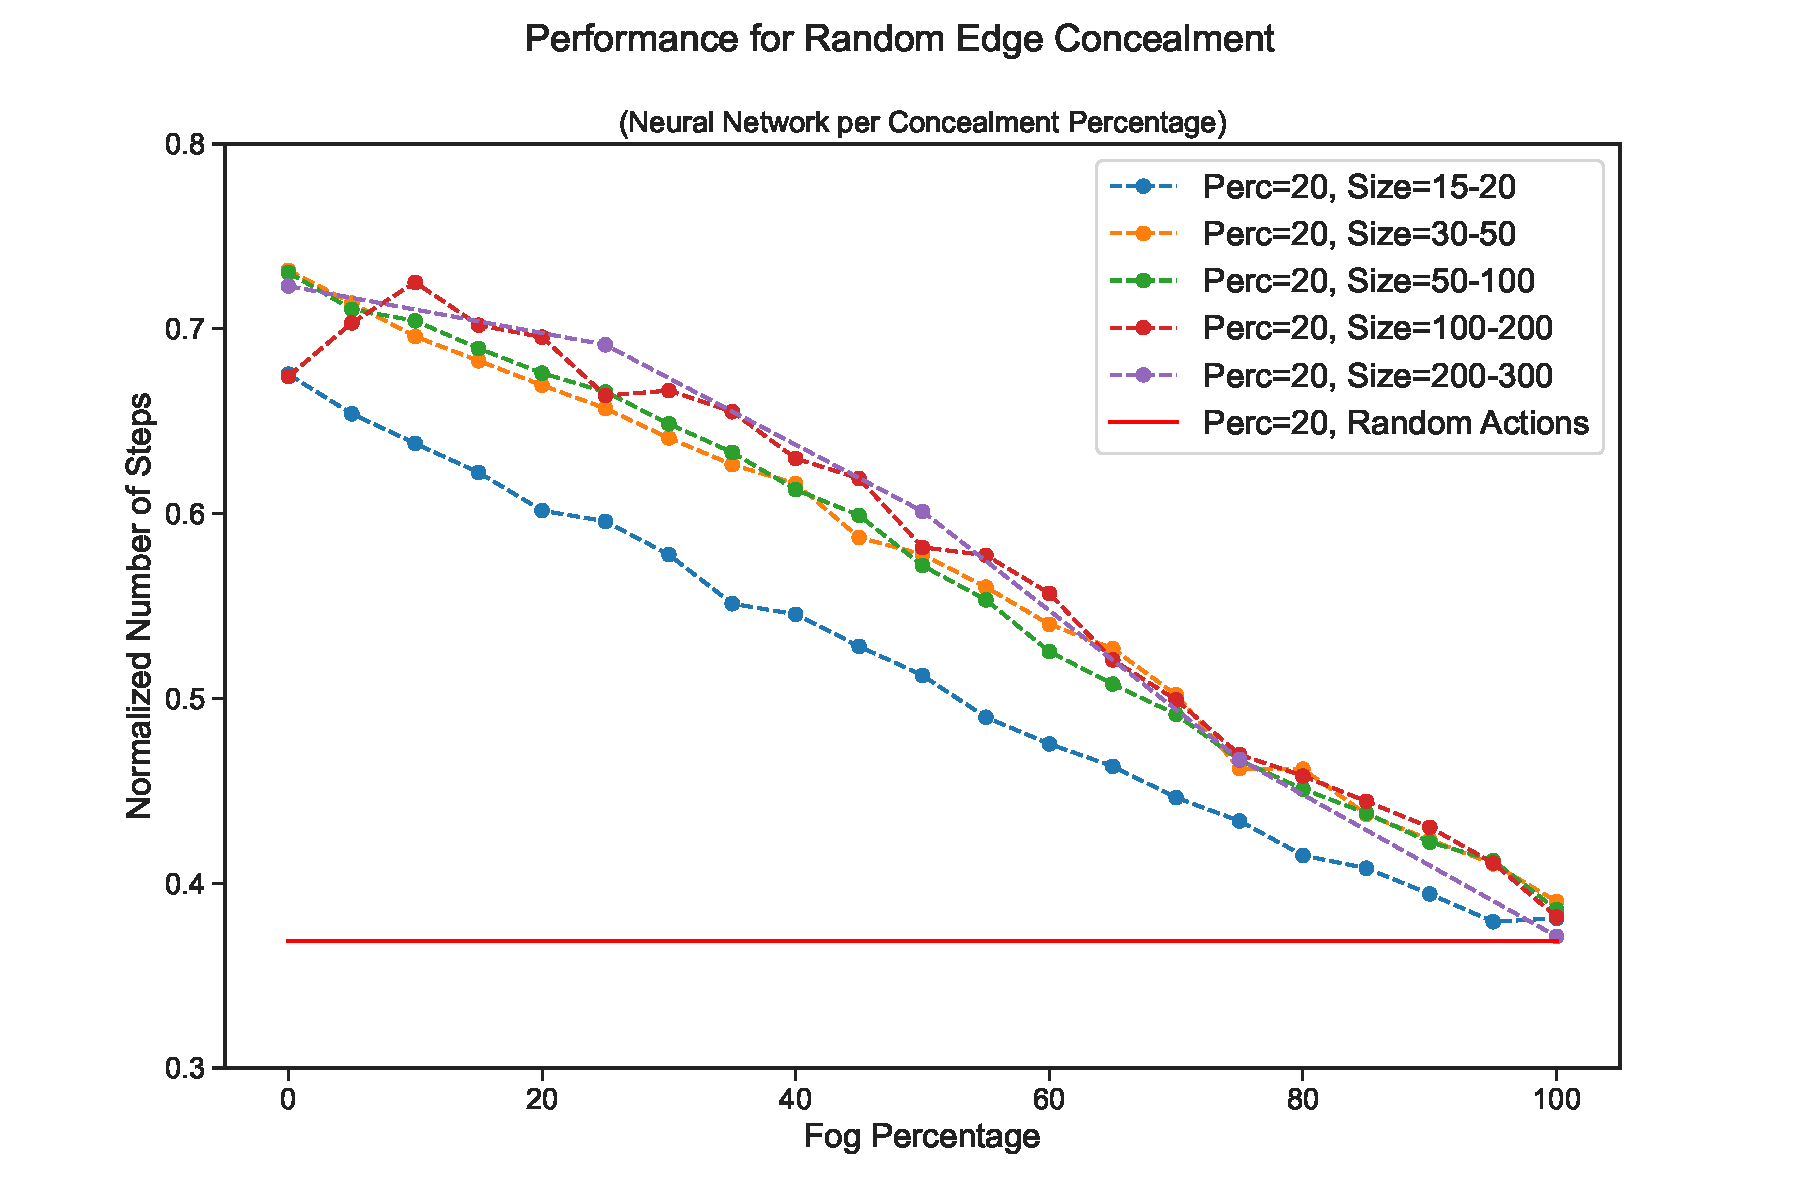
\includegraphics[scale=0.49]{Figures/percolation20_n200-300_k2-6_g2-3_random,all_fog.pdf}
    \caption[Caption Information]{\blindtext}
    \label{figure:random uniform (all models)}
\end{figure}

\begin{figure}[ht]
\sffamily\bfseries
    \centering
    % \textbf{Random Edge Concealment with Many Models}\par\medskip
    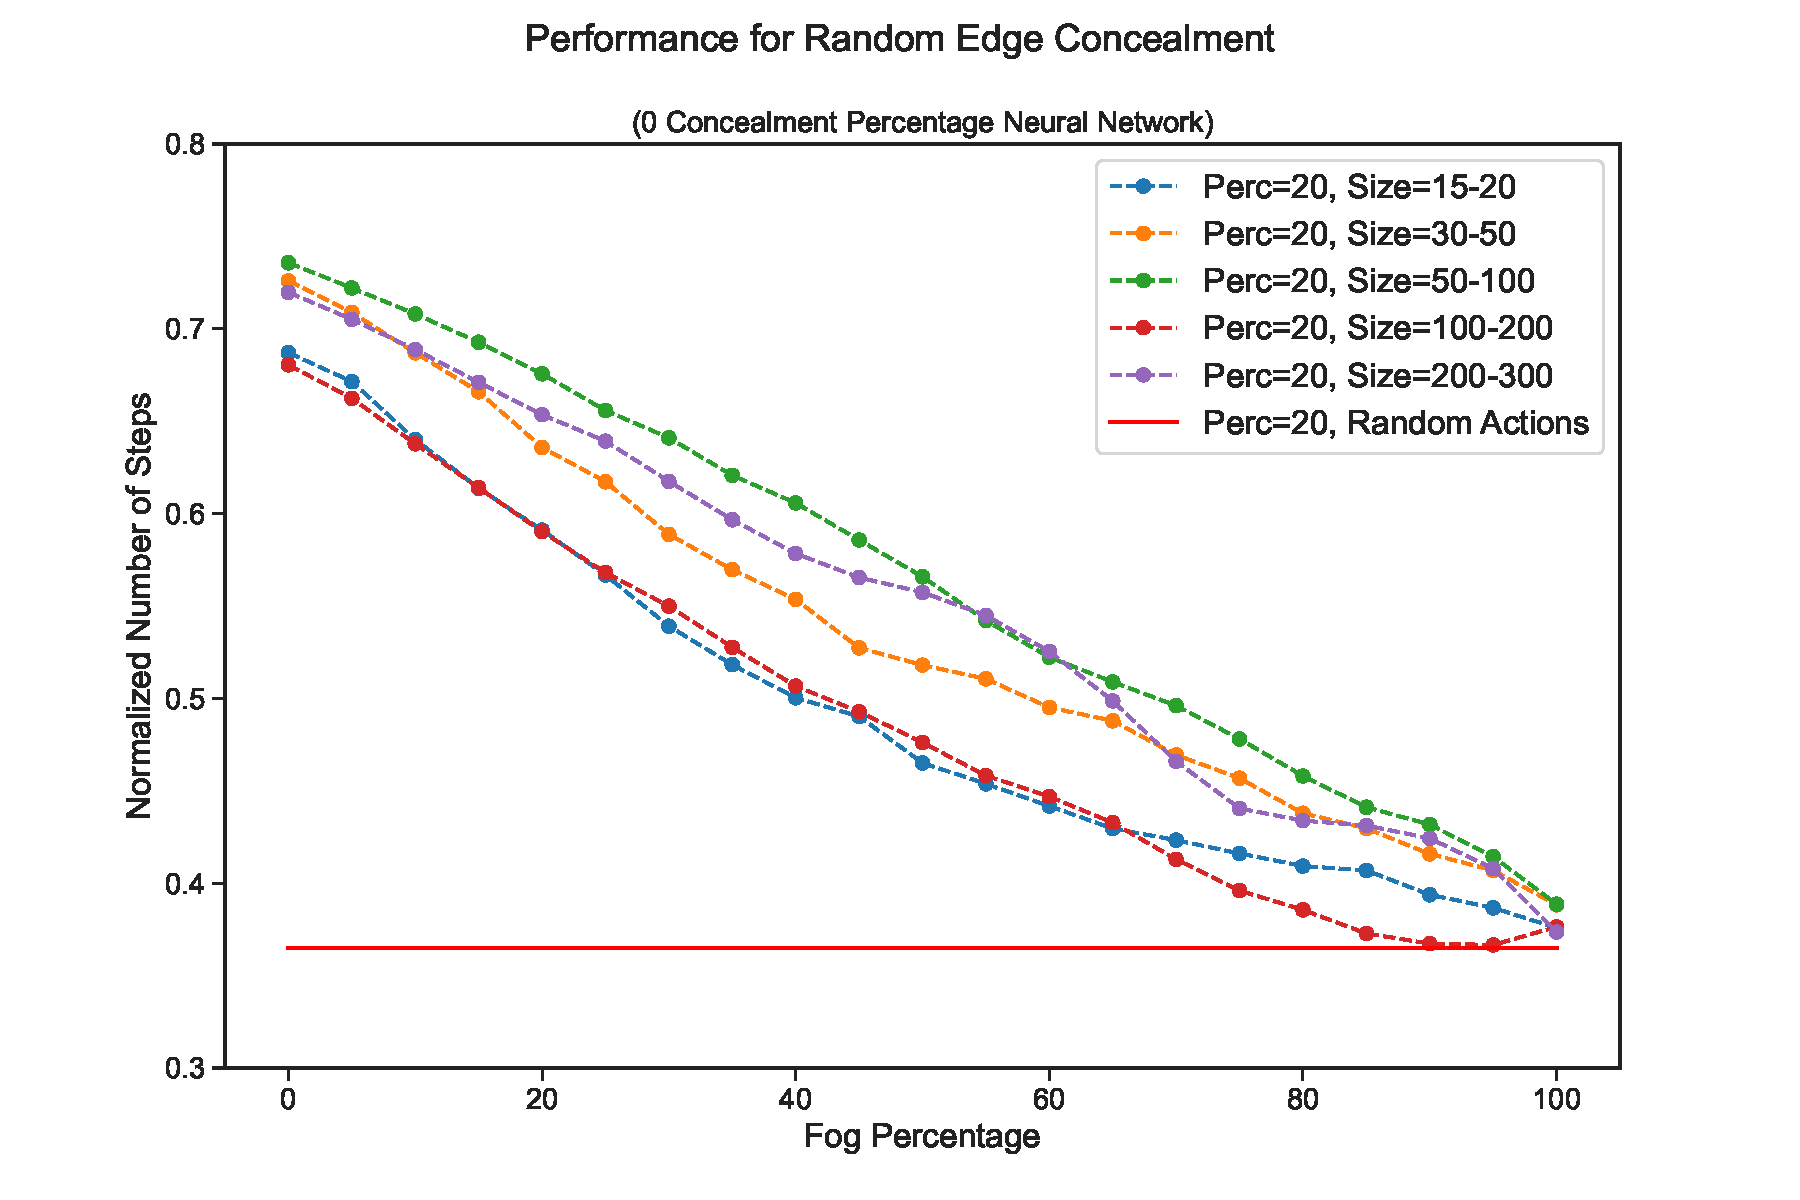
\includegraphics[scale=0.49]{Figures/percolation20_n200-300_k2-6_g2-3_p0.0_random,constant_fog.pdf}
    \caption[Caption Information]{\blindtext}
    \label{figure:random uniform (0 model)}
\end{figure}

\FloatBarrier
\clearpage
\subsection{Tabulated Performances}
% Random Edge Concealment
\begin{table}[ht]
    \centering \footnotesize
    \begin{tabular}{||c | c c ||} 
        \hline
        Network Size & \hyperref[figure:random uniform (all models)]{Area (All Models)} & \hyperref[figure:random uniform (0 model)]{Area (0.0 Model)}\\ [0.5ex] 
        \hline\hline
        15-20 & \gradient{0.13275} & \gradient{0.12930} \\ 
        \hline
        30-50 & \gradient{0.18738} & \gradient{0.17184} \\
        \hline
        50-100 & \gradient{0.18663} & \gradient{0.20129} \\
        \hline
        100-200 & \gradient{0.20822} & \gradient{0.12452} \\
        \hline
        200-300 & \gradient{0.20805}$\ast$ & \gradient{0.18448} \\ [1ex] 
        \hline
    \end{tabular}
    \caption[Caption information]{\blindtext}
    \label{table:uniform random}
\end{table}

% Discussion and Conclusion
% \clearpage
% % \addcontentsline{toc}{section}{Discussion}
\section{Discussion and Conclusion}
\vspace{-3em}
\subsection{Discussion}
\vspace{-2em}
\hspace{\parindent} \blindtext

\newpage
\vspace{-2em}
\subsection{Conclusion}
\vspace{-2em}
\hspace{\parindent} \blindtext


% References
\newpage
\addcontentsline{toc}{section}{References}
\section*{References}
\vspace{1em}
\pagestyle{fancyArabic}
% \vspace{-4em}
\bibliography{references.bib}
\bibliographystyle{naturemag}
% \nocite{*}

\end{document}